
% Due Date: 7/4/14

\chapter{Distributed Execution}
\label{chapter:distributed}
The third stage %(or second depending on mapping decisions) 
of the Legion task pipeline is the distribution stage.  
The distribution stage entails moving
a task and any necessary meta-data to the target node
on which the task is assigned to run by the mapper
that owns the task. The collection of mappers that own
a task also have control over whether the task is mapped 
{\em locally} (on the node on which the task originated) 
or {\em remotely} (on the target node).  This decision 
determines the ordering of the mapping and distribution 
stages  of the pipeline. If a task is assigned to a remote
node, the decision also determines what meta-data
must be moved in conjunction with the task.

In order to facilitate the distributed execution of
Legion tasks, the runtime must operate similarly to
a distributed system that is capable of reasoning 
about partitioned meta-data structures. In this
chapter, we describe the algorithms necessary for
allowing the Legion runtime to support distributed
execution of Legion applications (with the caveat
that we omit discussion of resiliency to
Chapter~\ref{chapter:resilience}).  We begin
in Section~\ref{sec:messaging} by describing 
the way messages are communicated between nodes
and the invariants supported by the communication
model. Section~\ref{sec:taskdist} describes how
both individual and index space tasks perform
the distribution stage of the task pipeline.
In Section~\ref{sec:distshape} we detail
how region tree data structures are migrated
through a distributed address space.  Finally,
we cover the details of how Legion supports
distributed physical contexts for parallel
mapping of non-interfering tasks in 
Section~\ref{sec:distctx}.

\section{Messaging Interface}
\label{sec:messaging}
The Legion high-level runtime operates on top of
the low-level runtime, therefore there is no 
explicit mechanism for the high-level runtime to 
send messages between two nodes.  Instead data 
can be moved in one of two ways: explicit copies 
or task launches on remote processors. Explicit copies 
are done  between physical instances and are optimized 
for moving data structures in bulk. The low-level 
runtime implements these copies efficiently using
asynchronous one-sided RDMA transfers. Alternatively,
task launches on remote processors can be 
accompanied with an un-typed buffer of data that 
is copied along with the task to the remote node.  
In general, the un-typed buffer is only used for 
capturing task arguments and should be relatively 
small. The low-level runtime implements remote
task launches using asynchronous active messages
supported by the GASNet API\cite{GASNet02}. The 
size of the buffer determines the size of the active
message required: either small (less than 128B), 
medium (less than about 8KB depending on hardware),
or large (anything greater than the medium size).
Pre-allocated buffers of pinned memory is maintained
by GASNet for small and medium active messages, making 
them considerably faster and lighter-weight than long 
active messages.

The Legion programming model encourages bulk transfers
of data and therefore all application data is always
moved by copies between physical instances. However,
determining the best approach for moving meta-data
is not as obvious. Region tree data structures are
large and could therefore benefit from being moved
in bulk.  However, in practice, our implementation
of distributed region trees (described in 
Sections~\ref{sec:distshape} and \ref{sec:distctx})
rely on an eventual consistency model that 
maintains persistent state on all nodes and relies
on sending fewer small updates instead of 
re-sending large bulk data structures each time
they are needed on a remote node. The Legion high-level
runtime therefore relies on sending tasks to remote 
processors as the primary communication mechanism 
for internal meta-data.

\subsection{Ordered Channels}
\label{subsec:channels}
While the Legion runtime uses remote task launch
as its primary communication mechanism, it does
so in a disciplined way.  Specifically, we create
the abstraction of an {\em ordered channel} for all
messages between a pair of nodes.  Ordering all
messages between a pair of nodes provides a useful
invariant for reasoning about the coherence of distributed
data structures.  In the case of the Legion runtime,
by knowing that all messages from one node to another 
are ordered, we will be able to develop a novel algorithm
for distributed garbage collection of physical instances
in Chapter~\ref{chapter:garbage}.

To implement our ordered channels, we create 
{\em message manager} objects on each node for 
sending messages to destination nodes.  Message
managers provide a thread safe interface that 
serializes all message requests from any thread running
on a node. In order to serialize messages to the
remote node, each message manager remembers the 
termination event of the most recent message.
This event serves as the
precondition for the next message to be run.
Message managers also handle all incoming messages
from the remote node that it is responsible
for managing.

In order for Legion to remain scalable, message managers
are lazily instantiated.  In the worst case, every node
in the system will attempt to talk to every other node
in the system.  If there are $N$ nodes in the system,
this will require each node to instantiate $N$ message
managers, ultimately requiring $N^2$ message managers
across all nodes.  Since message managers maintain some
state and a buffer for sending messages, this can result
in a significant cost of memory.  In practice, 
most nodes only talk to a subset of other nodes in the
machine.  Therefore, the Legion runtime only instantiates
a message manager for a destination node when either
it is requested as a target, or it receives a message 
from the remote node. 

\subsection{Deferred Sends}
\label{subsec:deferredsends}

While many of the messages sent by Legion are small
update messages, it is possible to defer many messages
for a short period of time and to aggregate many small
messages into larger messages that gain back some
of the efficiency of bulk data movement. The message
manager interface allows other components of the Legion
runtime to send messages and to indicate whether these
messages must be {\em flushed} (sent immediately) or
whether they can be deferred for a short period of
time. The message manager maintains a small buffer
for aggregating messages.  This buffer is intentionally
sized to target the maximum size of GASNet medium
active messages (usually between 8KB and 16KB). 
The message manager attempts to aggregate as many
message as possible into this buffer until either
the buffer fills up or a message that needs to be
flushed is requested, at which point the aggregate
message is sent. On the remote node, the message
manager that receives the aggregate message then
unpacks the smaller messages and invokes the 
proper handler. 

The message manager API is also intelligent 
enough to handle message requests that are bigger 
than its buffer size, breaking them up into smaller 
messages that fit into GASNet medium active
messages. By breaking up larger active messages
into slightly smaller ones, we can get data
moving through the network earlier, both reducing
latency and improving communication parallelism.
Note that even though messages are serialized
by low-level event dependences, those dependences
are handled by the remote node, meaning that the
active messages for those tasks can be in-flight
in the network simultaneously. Ultimately, the
message manager interface allows the Legion runtime
to strike a good balance between optimizing for
message throughput and latency by targeting 
GASNet medium sized active messages. The message manager 
interface also simplifies the implementation of other
runtime components, allowing them the illusion
of sending many small messages, that are ultimately
aggregated into larger messages.

\section{Task Distribution}
\label{sec:taskdist}
In practice, the mapping stage of the task pipeline
can actually be thought of as two separate
stages: the premapping stage and the actual 
mapping stage (see Chapter~\ref{chapter:physical}).
The premapping stage must always be done on the
origin node where a task was created. However, the
actual mapping can be performed either on the 
node where the task was created (locally) or on
the node where the task is going to be run (remotely).
In this section we discuss the implications of the
how both individual (Section~\ref{subsec:singledist})
and index space (Section~\ref{subsec:indexdist}) tasks
are distributed and actually mapped. In 
Section~\ref{subsec:stealdist}, we discuss how task
stealing is incorporated into task distribution.

\subsection{Single Task Distribution}
\label{subsec:singledist}
For single tasks, the distribution stage is fairly
straightforward.  Figure~\ref{fig:singletaskdist}
shows the distribution pipeline for an individual task
launch including the extra detail of physical traversals
from Chapter~\ref{chapter:physical}. After the task 
is finished premapping all of its regions, it first 
checks to see the mapper has selected for it to be 
locally or remotely mapped.  If the task is to be 
locally mapped, then the mapping is performed, the 
mapped regions are recorded, and the task is sent
to the target node where it is launched onto the
specified processor. If the task is to be remotely
mapped, then the task is sent to the
target node. If the task is not eligible for stealing
(see Section~\ref{subsec:stealdist}), then the 
physical region tree state necessary for mapping
the task is eagerly sent along with the task. If 
the task is eligible for stealing we defer sending
the region tree meta-data until we know for sure that
a task will attempt to map on a specific node.
(We discuss the movement of physical region tree
data in further detail in Section~\ref{sec:distctx}.)
When the task arrives on the target node, it is
placed in the ready queue for its intended processor.

\begin{figure}
\centering
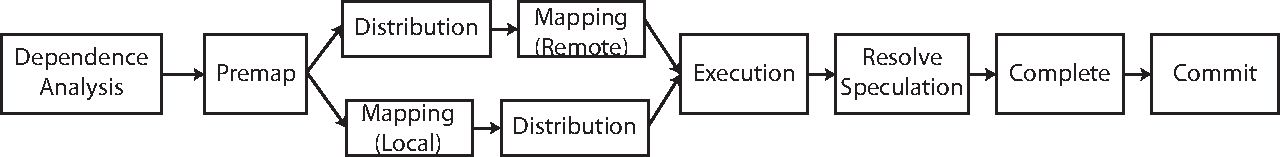
\includegraphics[scale=0.7]{figs/IndividualTaskPipeline.pdf}
\caption{Individual Task Pipeline\label{fig:singletaskdist}}
\end{figure}

Once a task is placed in the ready queue for the
target processor, then the mapper associated with
that processor can decide to either map the task
or to send it to another processor to be mapped.
If the mapper decides to map the task, then the runtime
first checks to see if the necessary meta-data
is resident.  If the region tree meta-data is not
local, then a request is sent to the owner node of
the task for the necessary state. The owner node
handles these requests and replies with the necessary
region tree meta-data. Once the meta-data arrives
the task can be mapped. If the meta-data is already
resident, the task is immediately added to the list
of tasks to map.

Alternatively, a mapper may also decide to continue
forwarding a task on to an additional processor.
A mapper might choose to make this decision if the
processor that it is managing is overloaded and it
knows of other processors with less work to perform.
Under these circumstances, even if the task has
been marked not eligible for stealing, the remote
state information is not automatically forwarded.
While it is useful to forward state eagerly the 
first time to reduce latency, if a task is moved
multiple times before being mapped, then the 
cost of moving the state outweighs the latency
savings. When the task ultimately does map, it
will first need to request the necessary region
tree meta-data from the owner node. While this
does add latency, it does reduce the overhead
of moving the task multiple times as the meta-data
only needs to be moved once from the owner node
to the node where the task is ultimately mapped.

\subsection{Index Space Task Distribution}
\label{subsec:indexdist}
Figure~\ref{fig:indextaskdist} shows the more detailed
pipeline for the stages of an index space task launch.
Index task distribution is more complicated than
for single tasks.  The reason for this is that
index space task launches create many sub-tasks
with a single call. To handle all of these tasks,
the distribution stage for index space tasks 
contains a sub-stage called {\em slicing}. Slicing
allows the mapper to break apart an index space
task launch into {\em slices} that describe a
subset of tasks in the original index space task
launch. Slices are created by the {\tt slice\_domain}
mapper call, which queries the mapper object 
to break apart an index space task into subsets of
tasks (although the mapper is not required to break 
apart an index space, and can create a single slice
that describes the entire set of tasks). Slices
act as the unit of reasoning about distribution 
for index space task launches, with all tasks
within a slice being moved together. By grouping
tasks into slices, the runtime can deduplicate
much of the meta-data necessary for moving sets
of tasks between nodes. 

\begin{figure}
\centering
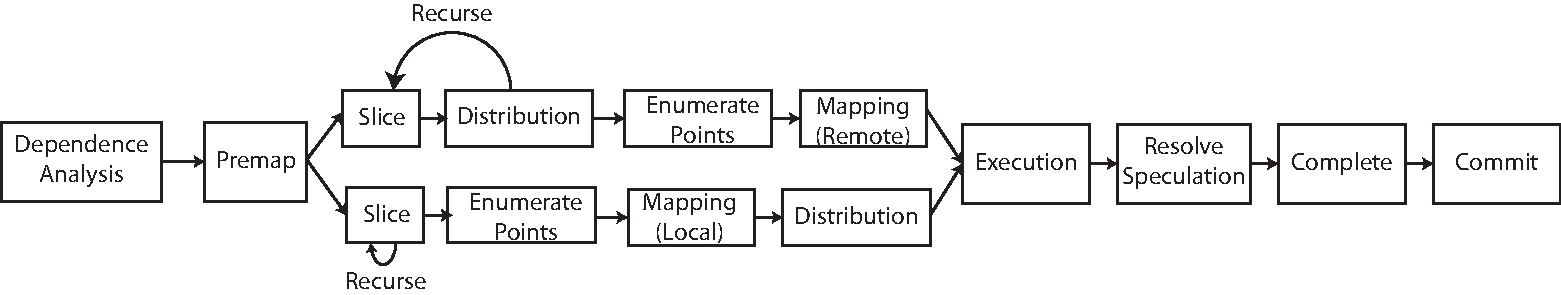
\includegraphics[scale=0.57]{figs/IndexTaskPipeline.pdf}
\caption{Index Task Pipeline\label{fig:indextaskdist}}
\end{figure}

In some cases, index space task launches can 
consist of very large numbers of tasks that need
to be distributed throughout an entire machine
that may contain thousands of nodes. To make
this process efficient, the slicing stage 
supports hierarchical division.  When a slice
is created, the mapper chooses two values for
the slice object: a target processor and a
boolean value indicating whether the slice
should be recursively sliced. If the mapper
asks for the slice to be recursively divided,
then when the slice arrives on the target
node, the mapper for the target processor is
invoked with the {\tt slice\_domain} call
to perform the recursive slice operation.
Ultimately it is up the mapper objects of
a task to determine how many times and how
finely an index space task is divided.

After slicing is complete, slice objects
are added to the ready queue, similar to 
individual tasks. Slices are the operations 
that traverse the pipeline, with the original 
index task operation waiting to complete
the final three stages of the pipeline until 
all of its constituent slices have completed 
the equivalent pipeline stages.
Slices behave like individual tasks until
they are ready to be mapped. The mapper that 
owns a slice can choose to map it onto its
processor or send it to another process to
be mapped. Slices can also be marked eligible
for stealing, as we will describe in 
Section~\ref{subsec:stealdist}. Once a slice
is ready to be mapped, the runtime enumerates
all the points in the slice, and generates
a {\em point task} for each point in the
slice. Each of these point tasks are then
mapped individually using the same routines
as individual tasks. 

Similar to individual tasks, an index space
of tasks can also be mapped both locally
and remotely. In the case of local mapping,
slicing is performed first, but none of the
slices are sent remotely until each of the
points within each slice have been mapped.
For remote mappings, slicing is performed
first, allowing slices to be moved throughout
the machine.  Once a slice is ready to be
mapped, it sends a request to the owner
node for the region tree meta-data necessary
to perform the mapping. The owner node
responds with this information, allowing
the slice to be mapped. Note that, unlike
individual tasks, region tree meta-data
is not eagerly sent to any nodes as part
of the slicing process.  The reason for this
is that it is common for slices to be
both recursively sliced and moved; therefore,
we avoid the cost of moving the meta-data
by lazily sending it only when it is 
explicitly requested.

\subsection{Distributed Stealing}
\label{subsec:stealdist}
While the distribution phase of the task
execution pipeline allows to tasks to be
pushed to their target processors (as 
we described in the previous two sections),
the distribution phase also allows tasks 
to be pulled to processors, with little or
no work, through stealing. By supporting both
push and pull models of task migration, 
Legion allows mappers sufficient flexibility
for expressing optimal ways of mapping a
particular application onto a target
architecture.

To support stealing, Legion allows mappers
to designate tasks as eligible to be
stolen by setting the {\em spawn} flag
in the {\tt select\_task\_options} mapper
call\footnote{The choice of {\em spawn} as the flag
was inspired by the semantics of the Cilk
language\cite{Cilk98}.}. While stealing in many
other programming models is done implicitly by
the runtime, stealing in Legion is directed by 
mappers because it impacts the performance 
of an application. Mappers can send steal requests 
to  any other mappers with the same ID on
different processors. Note by restricting steal
requests to other mappers with the same ID
we ensure that a task will always be mapped
by the same kind of mapper, albeit on different
processors. Unlike many stealing systems,
a steal request does not guarantee that a
steal will succeed.  Instead of having the
runtime automatically decide which tasks
are stolen by a steal request, the obvious
potential performance impacts mandate that
the decision be made by the mapper object.
Each steal request is therefore converted
by the runtime into a mapper call asking
the target mapper which (if any) of the 
eligible tasks that it owns are permitted
to be stolen. The mapper is free to specify
none, all, or a subset of its eligible tasks.
In order to make such a decision the mapper
can introspect information such as the location
of physical instances available for different
tasks that reveal locality information. We
discuss these considerations further
when we describe the full mapping interface
in Chapter~\ref{chapter:mapping}.

One important detail regarding stealing is
that only eligible tasks still in the
ready queue for a specific mapper can be
stolen.  Once a task has been mapped, then
it is guaranteed to execute on the target
processor and it cannot be stolen.  For mappers
that choose to employ stealing as a means
for performing task migration, there exists
a natural tension between mapping tasks
early to get any precondition operations in 
flight, and deferring mapping to achieve better 
load balance through stealing. To aid
in these decisions, mappers are given detailed
information regarding the number of queued
tasks on each processor allowing them to
make informed decisions about when to map
tasks. Importantly, all such decisions regarding
when to map tasks and when to permit stealing,
are under mapper control, ensuring that there
is no implicit decisions made by the runtime
that may impact performance.

Since stealing in Legion is primarily designed
to migrate tasks between nodes, Legion does
provides some additional support for avoiding
unnecessary steal requests.  When a steal fails,
Legion blacklists the target processor as one in 
which a steal has failed from the source processor.
No steal requests from the mapper of the source
processor will be allowed to be sent to the mapper 
of the target processor until the mapper on the target 
processor receives additional tasks that are
eligible for stealing in its ready queue.  The
runtime also records all the failed steal attempts
at a given processor.  When new tasks that are
eligible for stealing are added to the ready
queue, the runtime sends advertisements to all the
previously failed stealing processors.  These
advertisements remove the processor from the
blacklists of the attempted thieves.

Finally, while stealing in Legion will work between
any pair of processors, it works best between
different nodes, where it is more difficult
to achieve load balance. Task migration between
processors within a node is implemented in a fast
way that requires no copying of data.  However,
it is often more efficient to perform load-balancing
within a node using light-weight processor groups
that we discuss in Chapter~\ref{chapter:mapping}.

\section{Distributed Region Trees}
\label{sec:distshape}
While a Legion application is executing, it is 
free to dynamically create index spaces, 
field spaces, logical regions, and partitions. Each
of these operations are initially invoked by
a task on a single node, meaning that the
shape of the index space trees, field spaces, and
region trees are initially unknown to other nodes
immediately after creation. When a task is to be 
mapped remotely, it is the responsibility of the 
runtime to guarantee that the necessary index tree
and region tree shape information exist on the remote 
node where the mapping is to be performed. In this section 
we describe how the runtime maintains this 
guarantee efficiently by lazily moving region
tree shape information.

\subsection{Leveraging Lazy Tree Instantiation}
\label{subsec:lazytree}

In order to map a task remotely, the state
for performing the mapping must be sent to
the target node.  Before the state can be
sent, the runtime first checks to see which
region tree shape information must be sent
to instantiate the necessary region tree
data structures on the remote node for storing
the state information.  For each of the region
requirements requested by a task, the runtime
checks that necessary region tree shapes
can be created on the remote node. The only
traversals that are performed remotely are
the mapping traversal and the instance view
traversal.  Therefore for each region
requirement of the task, the runtime must 
ensure that the node corresponding to the
requested logical region and all sub-trees
are sent to the remote node. Additionally, 
because some instance view trees for physical
instances may contain views from parent logical
regions, all logical regions that are ancestors
of the requested logical region must also be
sent to the remote node.

While this may initially sound like a 
considerable number of region tree nodes
to send, we cut the number of nodes that
must be sent in half by leveraging the
lazy region tree instantiation supported
by the runtime (see 
Section~\ref{subsec:logicalshape}). 
Instead of having to send both the region
tree nodes as well as their corresponding
index space tree nodes, we only need to
send the necessary nodes from the index space
tree and the root node of the logical
region tree. This is sufficient from
the perspective of the remote node to 
instantiate the remaining parts of
the region tree when needed, thereby reducing 
the amount of data that must be sent
when moving a region tree to a remote node
by half.

\subsection{Creation and Deletion Sets}
\label{subsec:createsets}

To further reduce the amount of data that
must be sent when moving tasks between
nodes, all index space tree and logical
region tree nodes memoize the set of
other nodes in the machine to which they
have been sent. We call this set the 
{\em creation set}, and it records which
nodes in the machine know about the creation
of the index space tree node or region tree
node from the perspective of the local node.
It is possible that this set is stale and
does not accurately represent all the nodes
in the machine that are aware of the existence
of a node. However, this lack of information
can only result in duplicate sends of region
tree and index tree data. In practice these
duplicate sends are rare, and when they do
occur, the sending node is immediately added
to the creation set of all region tree and
index space nodes on the destination node,
to avoid further duplication.

In addition to creation sets, both region
tree nodes and index space tree nodes also
maintain deletion sets for tracking which nodes 
have been notified of the deletion of a node. 
Since node deletions are deferred
(there may be sub-tasks still using the node),
deletions of nodes in both the index space trees
and region trees do not immediately delete a
node, but instead simply mark it as deleted.
As the deletion propagates and removes privileges
working its way back up the task tree, the 
corresponding deletion information is only sent
to the proper nodes and only when the destination
node is unaware of the deletion.

To store both creation and deletion sets the
runtime uses a {\em node mask} data structure
that relies on the same base bit mask 
implementation as field masks (see
Section~\ref{subsec:fieldmasks}). However,
the upper bound on the number of entries in a
node masks is determined by the number of nodes
in the machine instead of the maximum number of
fields in a field space. While these node masks 
require $O(N)$ memory storage (in bits), 
they make checking for elements in the set $O(1)$, 
which is important since the common operation is 
traversing a tree to see which region tree and 
index space tree nodes still need to be sent to 
a destination node.

\subsection{Distributed Field Allocation}
\label{subsec:distfields}
The final aspect of maintaining distributed
region tree data structures is handling dynamic
field allocation\footnote{Dynamic allocation of
rows in unstructured index spaces is handled
by the low-level runtime.}. Each runtime instance 
statically partitions a space of field names for 
each field instance, allowing them to be able to
dynamically allocate field IDs without needing
to communicate with other runtime instances.
When a field is allocated on a specific node
it is given a unique ID, but it is not sent
to any other nodes.  Instead when a field space
is sent to a node, it sends all the field IDs
that it knows about to the target node. If the
field space already exists on the destination
node, only the newly allocated fields are sent.
Upon receipt of an update of newly allocated 
fields, the runtime always checks that the 
upper bound on the maximum number of fields
in a field space has not been exceeded (see
Section~\ref{subsec:fieldspace} for a description
of the upper bound).

The difficult part of this distributed allocation
scheme is maintaining a mapping of field IDs
in a field space to indexes in the field masks.
Each node maintains its own mapping. All nodes
coordinate on a scheme in which they attempt to
allocate fields at indexes that are equal to their
node number modulo the number of nodes in the entire 
machine. When these locations are exhausted they
progress to their neighbors locations. Ultimately the 
goal is to maintain the same mapping across all nodes
so field masks can be directly unpacked and not
require a transformation when they are sent from
one node to another.

In some cases though, different fields will
be allocated to the same index in different nodes.
To handle this case, each field space maintains
a permutation vector for every other node in the
machine that describes the necessary transformation 
that must be applied to unpacked field masks
received from every other node. Permutations are
also stored as field masks and are implemented
efficiently using the sheep and goats algorithm
from \cite{HackersDelight}. In practice most of
these permutations are the identity function.
The runtime tracks whether a permutation is the
identity function or not so that the identity
case can be easily skipped.


\section{Distributed Contexts}
\label{sec:distctx}
One of the options afforded to the mapper of a
task is to map the task remotely. To map remotely,
the necessary region tree state for performing the
mapping, registration, and instance view traversals
from Chapter~\ref{chapter:physical} must be available
on the remote node. To satisfy this requirement
the Legion runtime must provide a distributed 
implementation of the region tree meta-data for a
physical context. In a distributed environment where
many tasks can be mutating the state of a physical
context in parallel on different nodes, maintaining
the consistency of the physical state is challenging.
In this section we detail the approach that enables
Legion to support distributed physical contexts on
multiple nodes in a consistent manner.

\subsection{Eventual Consistency}
\label{subsec:eventual}
In order to support distributed mappings of non-interfering
tasks within the same context on different nodes, Legion 
permits the physical context from the owner node to be
replicated on remote nodes.  This allows non-interfering
tasks to map in parallel on remote nodes. The challenging
aspect to this approach is that tasks mapping in parallel
may mutate the state of a physical context in different
ways. To be safe, we need a mechanism to guarantee that
these independent mutations can be reconciled at a later
point in time. This deferred reconciliation of data 
structures at a later point in time is called 
{\em eventual consistency} in the distributed systems
community literature.

The primary requirement for supporting eventual consistency
is that the types of data being stored are instances
of convergent replicated datatypes (CRDTs) \cite{CRDT09}.
A CRDT is a type that is defined by a set of (possibly 
unbounded) instances and a meet operator.  The meet
operator is required to be associative, commutative,
and idempotent. The crucial insight for supporting 
eventual consistency for distributed region tree contexts
is that the set of possibles states for 
sub-trees open in either read-only or reduce mode 
represent instances of a CRDT.

For example, consider a region tree (or sub-tree) rooted
by a logical region $R$ in a context. For a given field,
the state of the region tree can take on many potential
values defined by the valid instances and open parts of
the sub-tree. These different states of the tree rooted
at $R$ define the different elements in the CRDT. The
meet operator is then defined to be the union operator
that unifies any two states for the sub-tree rooted 
at $R$. It is important to note that this union operator
only works if the state of the tree rooted in $R$ is
open in read-only or reduce mode, as these privilege
modes can only open parts of the sub-tree or add new
valid instances.  Read-write privileges do not have
this property as they can close sub-trees and remove
valid instances which invalidates the commutativity
of the union operator. Defined in this way, Legion can
permit multiple distributed nodes to be mapped in parallel 
on distinct nodes for trees open in read-only and reduce
mode and later be able to reconcile the state of the 
physical context.

\subsection{Sending Remote State}
\label{subsec:sendstate}

State of a physical region tree for a physical
context is sent to a remote node in one of two
cases. First, it can be sent eagerly when an
individual task that is not eligible for stealing 
is sent to a remote node (see 
Section~\ref{subsec:singledist}). The second,
and more common case, is that a request is received
from a remote node for the physical state 
meta-data necessary for mapping either an
individual task or a slice of an index space
task. When these requests occur, the runtime 
locates the meta-data for the requesting task
(this data is always resident because requests
are only handled by the owner node where the task
was originally created). For each of the region
requirements for these tasks, the runtime traverses
the region tree from the region on which
privileges were requested through all open
sub-trees for the requested fields. This traversal
ensures that all the meta-data necessary for performing
the mapping, registration, and instance view 
traversals will be resident on the remote node.

During the traversal, the state of each node in 
the region tree is sent to the target node including 
the dirty fields, valid physical instances, and open
sub-trees. Only state for the fields being requested
by the region requirement are sent. Each state is
sent as a separate message that can be deferred
allowing the message managers (described in 
Section~\ref{subsec:channels}) to aggregate the
smaller messages into larger ones. The traversal
also keeps track of the necessary instance views
and instance managers that must be sent to the 
remote node for performing the traversal. After
the entire traversal is finished, the instance
view and instance managers are also sent to the
remote node.  Instance managers are always
sent in full, while instance views only need to
send the members of the epoch lists for the
fields being requested by the region requirement.

On the remote node, the messages are handled and 
unpacked into another physical context serves as a
clone of the physical context on the owner
node (note this context does not need to remain
a clone and can diverge from the owner node under
the conditions of CRDTs). Each message contains the 
logical region node for the state that is being unpacked,
allowing the state to be updated directly. It is
important to note that unpacking state is merged
into the existing state rather than overwriting
it as the context may already contain valid
data for other fields from another task that
mapped on the same remote node (see 
Section~\ref{subsec:persistence} for a detailed
description of persistent remote contexts). 
The remote node also handles messages for 
instance view and instance managers. Instance
managers and instance views are either updated
or created by the runtime to ensure that 
there exists a unique one on the node\footnote{
Instance managers are unique on a node, 
while instance views are unique within a 
context on a node.}.

After the traversal of all the region requirements
in the physical state has been completed, the owner 
node replies to the requesting remote node with a 
message indicating that all of the physical state
data has been sent.  This message is marked as being 
unable to be deferred, which causes the message 
manager to flush the ordered channel to the remote 
node. Since all messages between a pair of nodes 
are both sent and received in order, by the time 
the remote node observes the notification, all of
the necessary physical state has already been unpacked
in its region tree.  The runtime on the remote node
can then resume the mapping process for the task.

\subsection{Receiving Remote State Updates}
\label{subsec:receivestate}

When a task has finished mapping, it returns the
updated state of the region tree back to the origin
node of the task\footnote{There is an important interaction
with virtual mappings here: tasks with virtual 
mappings cannot return their state until they have
finished mapping all their child operations.}. While 
eagerly flushing meta-data back to the origin node
is not strictly necessary
(we could have opted to employ a distributed coherence
mechanism for tracking which nodes had valid state
for a specific fields of each region tree node), we 
decided on this approach in order to ensure a
simpler implementation\footnote{The analogy to modern
processors is the difference between a write-back
and a write-through cache. Eagerly flushing data is
like writing through the cache back to main memory.}.

To return the meta-data state back to the origin 
node, the runtime traverses the sub-trees for
all regions on which the task held privileges, and
sends back the state of these nodes. We currently
send back the entire state as it is relatively cheap
to represent.  Upon receiving the remote state on
the origin node, one of two operations is performed.
If the state is coming from a region requirement that
requested read-only or reduce privileges, the state
is unioned with the existing state on the owner node.
Performing a union is possible because the state of
the region tree under read-only or reduce privileges
is a CRDT (see Section~\ref{subsec:eventual}), allowing
states from distributed nodes to be safely merged.
Alternatively, if the state is returning from a sub-tree
on which the remote task had read-write privileges, 
then the existing state on the owner node is first
invalidated, and then the returning state is 
written as the new state. Read-write privileges
guarantee that there is only ever at most one task
mutating the state of that sub-tree at a time,
and the canonical version of that state is therefore
always the most recently written one.

In addition to returning state for region tree
nodes, state for the epoch user lists of instance
view objects is also returned.  Similar to returning
state for region tree nodes, whether or not the
state is merged or overwritten depends on the privilege
context under which it is being returned. If the
added users are being returned within a read-only
or reduce privilege context, then they are merged
with the existing set of users.  Otherwise, the
current epoch lists are invalidated for the fields
being returned, and the new users are added to the
lists as the new version of the epoch lists for
the returned fields.

\subsection{Persistence of Remote Contexts}
\label{subsec:persistence}

One important optimization implemented by the runtime
is deduplication of remote physical contexts. In
many cases, multiple sub-tasks from the same parent
task are sent to the same remote node to be mapped.
Often, these sub-tasks will request some of the same
state in order to map their regions. Under such 
circumstances, it is inefficient for the runtime to
send multiple copies of the same physical state to 
a remote node. Instead, the runtime deduplicates 
these requests by ensuring that at most a single 
copy of any physical context exists on any remote node.

On each node, the runtime tracks all of the physical
contexts that have been allocated, as well as 
whether the allocated contexts are for a task running
on the local node, or whether the contexts are remote 
versions of a context from a different node. If a context
is a remote version, then the runtime also tracks the
identity of the parent task on the owner node associated
with the remote clone context. When a task is
received to be executed and mapped remotely on a 
node, the runtime first checks to see if an existing
remote context has been allocated for the parent 
task. If it has, the child task is told of the appropriate
context so that it can use it as the target of any
remote state requests that are sent to the owner node.
If no such context exists, then a new remote clone
context is allocated and registered.  Any future
tasks that are sent to the node with the same parent
task are then guaranteed to re-use the same context.

The parent task on the owner node also tracks the
set of remote clone contexts that exist on remote nodes.
Individual region tree nodes in the context on the owner
node track the validity of state information for 
different fields on remote nodes. We discuss the
protocol for maintaining this validity in
Section~\ref{subsec:invalidate}. When the parent task
commits on the owner node, it is safe to infer that
there is no longer a need for the remote clone contexts
to be maintained.  At this point, the owner node sends
messages to all of the nodes that contain remote clone
contexts, instructing them to invalidate the remote contexts
and recycle them so that can be re-used for future tasks.

\subsection{Invalidate Protocol for Remote Context Coherence}
\label{subsec:invalidate}

Maintaining coherence of the distributed region tree 
state is a challenging problem. Not surprisingly, this
problem has a natural analog in modern hardware processors:
maintaining cache coherence. Modern hardware processors
support replication of cache lines whenever possible for different
processors in the same chip while still guaranteeing a 
total order on writes to the cache line. Legion relies on
a similar approach for maintaining coherence of the region
tree state within a physical context that have been replicated
throughout the nodes of a machine.

We considered two potential adaptations of cache coherence
protocols on which to base our Legion implementation.  Our
initial approach was based on an update protocol.  In an
update protocol, data initially resides on a single node.
As other nodes request data, they become subscribers. Any
updates to the data are eagerly flushed out to all of the
subscribers.  Our initial implementation based on an 
update protocol maintained a set of subscribers for each
region tree node.  While the update protocol performed well
at small node counts, it failed to perform well at larger
node counts.  At larger node counts, there are many
unnecessary update messages sent that ultimately are  
not used for mapping any future tasks in a specific
part of the region tree.

Our second design is based on an invalidation cache 
coherence protocol. In an invalidation protocol, remote
copies of the data are invalidated, and requests are
generated by the remote node to pull data from the owner
node (which always has a valid copy) to the requesting
node. Invalidation protocols scale better because they
move data lazily, which ensures that data is only moved
when it is actually going to be used. In our Legion 
implementation, each region tree node on the owner node
maintains a {\em directory} object (similar to the directory
maintained by distributed memory cache coherence protocols).
The directory stores two kinds of information for each field:
the {\em mode} it is in and for each field, the set of
nodes that contain valid versions of the state. Each 
field within a state can be in one of three modes 
corresponding to the different region privileges:
read-only, read-write, and reduce.  The read-only and
reduce modes permit multiple nodes to have valid copies
of the data simultaneously, while the read-write mode
permits at most a single other node to maintain a valid 
copy of the state.

Whenever a state transition takes place for a node within
a field, all outstanding remote copies are invalidated.
The invalidation is both recorded on the owner node and
on the remote nodes by messages sent from the owner node.
It is important to node that the owner node always maintains
a valid copy of the state for all fields of all nodes 
within a context because all tasks eagerly flush changes
to the region tree back to the owner node. In many ways
this approach is similar to write-through caches that always
flush data back to the backing memory so that the directory
owner always has a valid copy of the data. Remote nodes
can then request updated versions of the state for any 
set of region tree nodes when necessary.

\subsection{Distributed Futures}
\label{subsec:distfutures}

The final piece of distributed state within a context that
must be considered are futures.  Futures are local to the
context of the parent task in which they are created.
However, sub-tasks can request future values as arguments.
If these tasks are mapped to processors on remote nodes, 
it is the responsibility of the runtime to ensure that the
value of the future is propagated to the remote node
when the future completes.

To support this feature, the runtime implements {\em distributed
futures}.  Distributed futures operate in a similar manner
to instance managers (see Section~\ref{subsec:instmanagers}).
There is an owner distributed future created on the owner
node and clones can be created on remote nodes. Each
distributed future remembers the nodes where versions already
exist as well as the node that contains the original owner
node.  Distributed futures are registered with the runtime
to ensure that they are deduplicated within a node (guaranteeing
that at most one distributed future exists on each node).
Each remote distributed future registers itself with the
owner version on the owner node. When the owner distributed
future completes, it broadcasts out the value associated
for the future with any registered waiters on remote nodes.
If the owner distributed future receives any requests after
it has already completed, it immediately replies with the 
value of the future. When remote nodes receive the values
for the future, they also complete immediately and notify
any tasks that may have been waiting on them that they
are complete (usually done with low-level runtime events).
Distributed futures are reclaimed with the same garbage
collection algorithm as instance managers which is discussed
in detail in Chapter~\ref{chapter:garbage}.

